\documentclass[
    12pt,
    twoside,
    titlepage
]{article}

% https://tug.org/FontCatalogue/
% koristi sans serif font:
\usepackage[defaultsans]{droidsans}
\renewcommand*\familydefault{\sfdefault} %% Only if the base font of the document is to be typewriter style
\usepackage[T1]{fontenc}

\usepackage[
    a4paper,
    nomarginpar,
    margin=2.54cm,
    inner=3.54cm
]{geometry}

\usepackage[croatian]{babel}

\usepackage{blindtext} % debug: generiraj zamjenski tekst (Lorem ipsum...)

\newcommand{\accentColor}{DarkBlue} % akcent boja
% https://www.w3.org/TR/SVG11/types.html#ColorKeywords
% korištenje imenovanih boja (SVG 1.1 standard, osjetljiv na velika/mala slova):
\usepackage[svgnames]{xcolor}

\usepackage{fancyhdr}
\pagestyle{fancy}
\fancyhf{} % reset default header and footer
\renewcommand{\headrulewidth}{0pt}
\fancyfoot[LE,RO]{\thepage}

\usepackage[useregional]{datetime2}
\date{\DTMdisplaydate{2023}{10}{02}{-1}} % (-1 = ne prikazuj dan u tjednu)

\usepackage{emptypage}

\usepackage[dotinlabels]{titletoc} % točka poslije brojeva naslova u sadržaju
\usepackage{titlesec}
\pretocmd{\section}{\cleardoublepage}{}{}
\titleformat{\section}
    {\large\bfseries\color{\accentColor}}{\thesection.}{5pt}{}[{\titlerule[1pt]}]
\titleformat{\subsection}
    {\bfseries\color{\accentColor}}{\thesubsection.}{5pt}{}
\titleformat{\subsubsection}
    {\bfseries}{\thesubsubsection.}{5pt}{}

% \usepackage{showframe} % debug: prikaži obrube

\linespread{1.25}
\usepackage{indentfirst}

\usepackage{hyperref} % URL's
\hypersetup{
    colorlinks=true,
    linkcolor=black,
    urlcolor=DarkBlue        % color of external links
}
\urlstyle{same}

% \setcounter{tocdepth}{2}

\usepackage{graphicx}
\graphicspath{ {./images/} }

% \usepackage[skip=-10pt]{caption} % example skip set to 2pt

\usepackage{subcaption}
\DeclareCaptionFormat{custom}
{%
    \textbf{#1#2}\textit{\small #3}
}
\captionsetup{format=custom}

\usepackage{listings}

\usepackage{noto}
\usepackage[T1]{fontenc}

\lstdefinestyle{mystyle}{
    commentstyle=\color{DodgerBlue},
    keywordstyle=\bfseries\color{DarkBlue},
    % numberstyle=\color{Blue},
    stringstyle=\color{MediumBlue},
    basicstyle=\linespread{0.8}\ttfamily\footnotesize,
    breakatwhitespace=false,
    breaklines=true,
    captionpos=b,
    keepspaces=true,
    % numbers=left,
    showspaces=false,
    showstringspaces=false,
    showtabs=false,
    tabsize=2,
    frame=single
}

\lstset{style=mystyle}
\lstset{extendedchars=true, inputencoding=utf8,
literate      =        % Support additional characters
{á}{{\'a}}1  {é}{{\'e}}1  {í}{{\'i}}1 {ó}{{\'o}}1  {ú}{{\'u}}1
{Á}{{\'A}}1  {É}{{\'E}}1  {Í}{{\'I}}1 {Ó}{{\'O}}1  {Ú}{{\'U}}1
{à}{{\`a}}1  {è}{{\`e}}1  {ì}{{\`i}}1 {ò}{{\`o}}1  {ù}{{\`u}}1
{À}{{\`A}}1  {È}{{\`E}}1  {Ì}{{\`I}}1 {Ò}{{\`O}}1  {Ù}{{\`U}}1
{ä}{{\"a}}1  {ë}{{\"e}}1  {ï}{{\"i}}1 {ö}{{\"o}}1  {ü}{{\"u}}1
{Ä}{{\"A}}1  {Ë}{{\"E}}1  {Ï}{{\"I}}1 {Ö}{{\"O}}1  {Ü}{{\"U}}1
{â}{{\^a}}1  {ê}{{\^e}}1  {î}{{\^i}}1 {ô}{{\^o}}1  {û}{{\^u}}1
{Â}{{\^A}}1  {Ê}{{\^E}}1  {Î}{{\^I}}1 {Ô}{{\^O}}1  {Û}{{\^U}}1
{œ}{{\oe}}1  {Œ}{{\OE}}1  {æ}{{\ae}}1 {Æ}{{\AE}}1  {ß}{{\ss}}1
{ẞ}{{\SS}}1  {ç}{{\c{c}}}1 {Ç}{{\c{C}}}1 {ø}{{\o}}1  {Ø}{{\O}}1
{å}{{\aa}}1  {Å}{{\AA}}1  {ã}{{\~a}}1  {õ}{{\~o}}1 {Ã}{{\~A}}1
{Õ}{{\~O}}1  {ñ}{{\~n}}1  {Ñ}{{\~N}}1  {¿}{{?`}}1  {¡}{{!`}}1
{°}{{\textdegree}}1 {º}{{\textordmasculine}}1 {ª}{{\textordfeminine}}1
{£}{{\pounds}}1  {©}{{\copyright}}1  {®}{{\textregistered}}1
{«}{{\guillemotleft}}1  {»}{{\guillemotright}}1  {Ð}{{\DH}}1  {ð}{{\dh}}1
{Ý}{{\'Y}}1    {ý}{{\'y}}1    {Þ}{{\TH}}1    {þ}{{\th}}1    {Ă}{{\u{A}}}1
{ă}{{\u{a}}}1  {Ą}{{\k{A}}}1  {ą}{{\k{a}}}1  {Ć}{{\'C}}1    {ć}{{\'c}}1
{Č}{{\v{C}}}1  {č}{{\v{c}}}1  {Ď}{{\v{D}}}1  {ď}{{\v{d}}}1  {Đ}{{\DJ}}1
{đ}{{\dj}}1    {Ė}{{\.{E}}}1  {ė}{{\.{e}}}1  {Ę}{{\k{E}}}1  {ę}{{\k{e}}}1
{Ě}{{\v{E}}}1  {ě}{{\v{e}}}1  {Ğ}{{\u{G}}}1  {ğ}{{\u{g}}}1  {Ĩ}{{\~I}}1
{ĩ}{{\~\i}}1   {Į}{{\k{I}}}1  {į}{{\k{i}}}1  {İ}{{\.{I}}}1  {ı}{{\i}}1
{Ĺ}{{\'L}}1    {ĺ}{{\'l}}1    {Ľ}{{\v{L}}}1  {ľ}{{\v{l}}}1  {Ł}{{\L{}}}1
{ł}{{\l{}}}1   {Ń}{{\'N}}1    {ń}{{\'n}}1    {Ň}{{\v{N}}}1  {ň}{{\v{n}}}1
{Ő}{{\H{O}}}1  {ő}{{\H{o}}}1  {Ŕ}{{\'{R}}}1  {ŕ}{{\'{r}}}1  {Ř}{{\v{R}}}1
{ř}{{\v{r}}}1  {Ś}{{\'S}}1    {ś}{{\'s}}1    {Ş}{{\c{S}}}1  {ş}{{\c{s}}}1
{Š}{{\v{S}}}1  {š}{{\v{s}}}1  {Ť}{{\v{T}}}1  {ť}{{\v{t}}}1  {Ũ}{{\~U}}1
{ũ}{{\~u}}1    {Ū}{{\={U}}}1  {ū}{{\={u}}}1  {Ů}{{\r{U}}}1  {ů}{{\r{u}}}1
{Ű}{{\H{U}}}1  {ű}{{\H{u}}}1  {Ų}{{\k{U}}}1  {ų}{{\k{u}}}1  {Ź}{{\'Z}}1
{ź}{{\'z}}1    {Ż}{{\.Z}}1    {ż}{{\.z}}1    {Ž}{{\v{Z}}}1 {ž}{{\v{z}}}1
{Ž}{{\v{Z}}}1
% ¿ and ¡ are not correctly displayed if inconsolata font is used
% together with the lstlisting environment. Consider typing code in
% external files and using \lstinputlisting to display them instead.
}
\lstset{inputpath="./code/"}
\renewcommand{\lstlistingname}{Izvorni kod}% Listing -> Algorithm
\renewcommand{\lstlistlistingname}{Popis izvornih kodova}% List of Listings -> List of Algorithms

\lstdefinelanguage{JavaScript}{
  keywords={break, case, catch, continue, debugger, default, delete, do, else, finally, for, function, if, in, instanceof, new, return, switch, this, throw, try, typeof, var, void, while, with},
  morecomment=[l]{//},
  morecomment=[s]{/*}{*/},
  morestring=[b]',
  morestring=[b]",
  sensitive=true
}

\usepackage[nottoc]{tocbibind} % To include lists in the TOC
\usepackage{wrapfig}

\usepackage{pdfpages}

\usepackage{tabularx}

\usepackage{calc}

\newlength{\mytextwidth}
\newlength{\myline}

\def\Author{Ivan Dolovčak}
\def\Title{\textit{Web} aplikacija za izradu, rješavanje i statistiku ispita i obrazaca}

\usepackage{enumitem}


\begin{document}

\begin{titlepage}
    \begin{center}
        \Large
        Srednja škola Krapina
    \end{center}

    \vfill

    \begin{center}
            \normalsize \Author

            \vspace{0.5cm}

            \mbox{\huge\textbf{ZAVRŠNI RAD}}

            \vspace{0.3cm}

            \normalsize \Title
    \end{center}

    \vfill

    \begin{center}
        \normalsize
        Krapina, 2024.
    \end{center}
\end{titlepage}

\cleardoublepage

\begin{titlepage}
    \begin{flushleft}
        Srednja škola Krapina\\
        Šetalište hrvatskog narodnog preporoda 6\\
        49000 Krapina, Hrvatska\\
    \end{flushleft}

    \vfill

    \begin{center}
        \LARGE
        \textbf{\Title}\\

        \vspace{0.5cm}

        \Large
        \textcolor{\accentColor}{\textbf{Završni rad}}\\

    \end{center}

    \vfill

    \begin{flushleft}
        \normalsize
        \textbf{Zanimanje:} tehničar za računalstvo\\
        \textbf{Predmet:} Napredno i objektno programiranje\\
        \textbf{Mentor:} Stjepan Šalković, mag. inf. univ. spec. oec.\\
        \textbf{Učenik:} \Author, 4.AT\\
    \end{flushleft}

    \vspace{1cm}

    \begin{center}
        Krapina, svibanj 2024.
    \end{center}
\end{titlepage}


\tableofcontents

\newpage

\section{Uvod}

  \subsection{Problematika}

    Ispiti i obrasci su svakodnevnica obrazovnog i poslovnog okruženja. Napretkom
    tehnologije i digitalizacijom pojavila se ideja za automatiziranjem procesa
    izrade profesionalnih obrazaca i ispita. Tako su nastale prve (web) aplikacije
    za izradu, ali i obradu takvih dokumenata. Takve aplikacije su bile
    inspiracija za temu ovog završnog rada.

  \subsection{Tema}

    Tema završnog rada je web aplikacija za izradu, rješavanje i statistiku
    ispita i obrazaca. Nadalje u tekstu riječ \textit{dokument} se odnosi na
    obrase i na ispite. Aplikacijom je moguće izraditi dokumente s određenim
    postavkama: tip dokumenta (obrazac ili ispit), rok predaje, broj dozvoljenih
    pokušaja predaje i vidljivost dokumenta (javni, privatni ili skriveni).
    Nakon izrade dokumenta moguće je i mijenjati te postavke. Također je moguće
    i obrisati dokumente.

    Aplikacija pruža različite prikaze popisa dokumenata. Moguće je vidjeti
    vlastite dokumente, ali i pretražiti tuđe, te ih i rješiti (predati).

    Da bi krajnji korisnik/ca aplikacije mogao/la pristupiti svim mogućnostima
    aplikacije, potrebno se registrirati i prijaviti u aplikaciju. Korisnik/ca
    nakon prijave može mijenjati detalje svog profila (ime, prezime, korisničko
    ime i e-mail adresa) te izbrisati svoj profil.

    Također, korisnik/ca može mijenjati izgled aplikacije i bez da je
    prijavljen/a u aplikaciju. Moguće je odabrati jezik aplikacije (hrvatski ili
    engleski), temu (svijetla ili tamna) i proizvoljnu boju isticanja (engl.
    \textit{accent color}).

\section{Programski alati}

  \subsection{Uređivači izvornog koda}

    \subsubsection*{\textit{VSCodium}}

      \textit{VSCodium} je program uređivač izvornog koda koji je razvio
      Microsoft 2015. g. Vrlo je popularan, funkcionalan i prilagodljiv.
      Podržava otklanjanje grešaka, ugrađenu \textit{git} kontrolu, isticanje
      sintakse i automatsko dovršavanje koda. \textit{VSCodium} je inačica
      programa \textit{VSCode} iz koje je uklonjeno telemetrijsko prikupljanje
      korisničkih podataka. Izvorni kod programa je besplatan i otvoren.

      \begin{figure}[h]
        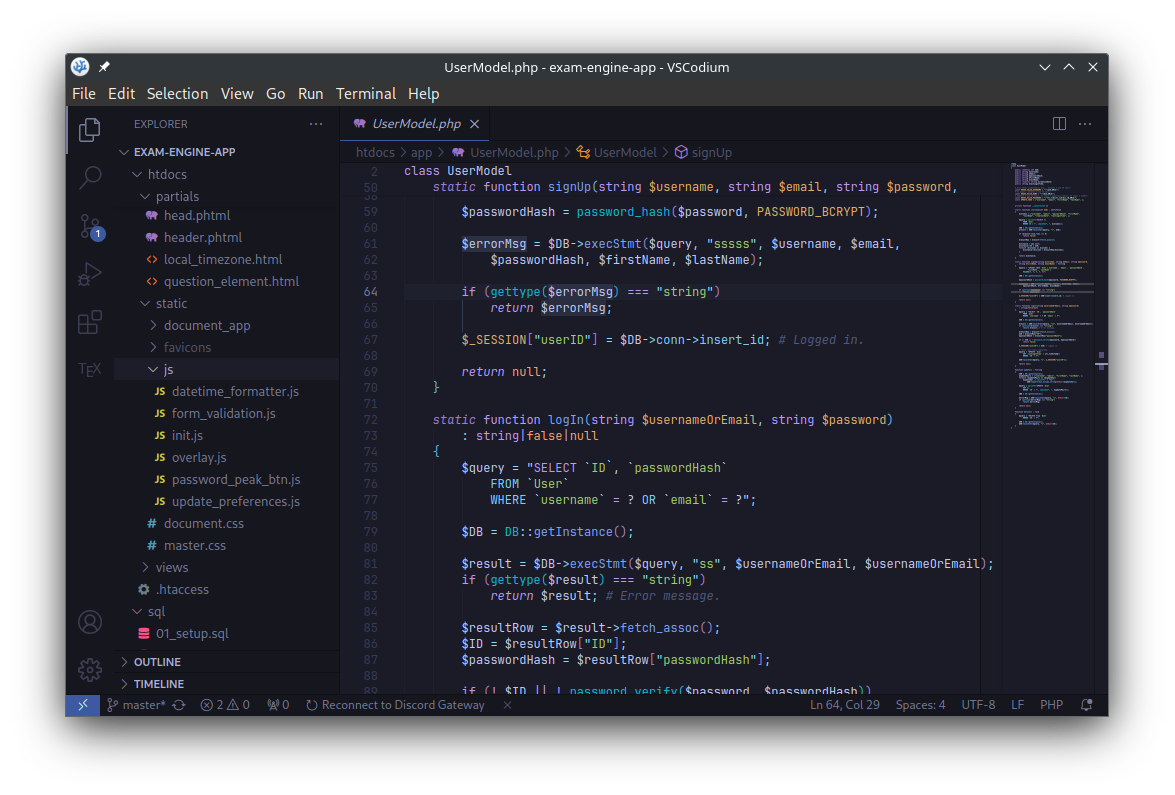
\includegraphics[width=\textwidth]{vscodium}
        \caption{VSCodium uređivač koda s otvorenim projektom.}
      \end{figure}

      \textit{VSCodium} sam koristio kao glavni uređivač teksta za cijeli
      projekt. Omogučio mi je brzo, organizirano i funkcionalno digitalno radno
      okruženje.

      \subsubsection*{\textit{vim}}

      \textit{vim} je program uređivač izvornog koda nastao 1991. g. Za razliku
      od \textit{VSCodiuma} koji ima grafičko korisničko sučelje (GUI),
      \textit{vim} ima isključivo tekstualno korisničko sučelje (TUI).

      \textit{vim} sam koristio isključivo za uređivanje pojedinačnih datoteka
      izvan projekta i malih konfiguracijskih datoteka (npr. Apache
      konfiguracija).

  \subsection{Kontrola izvornog koda}

    \textit{git} je program za upravljanje izvornim kodom nastao 2005. g.
    Njegov kreator Linus Torvalds je ujedno i voditelj razvoja Linux
    operativnog sustava.

    Pomoću \textit{gita} sam spremao i bilježio napredak svog projekta.
    Također sam objavio izvorni kod svoje aplikacije na web sjedištu
    \textit{GitHubu}, koji nudi uslugu tzv. \textit{hostinga} izvornog koda,
    što je ujedno služilo za čuvanje sigurnosne kopije.

  \subsection{Terminal}

    \textit{kitty} je napredni Linux emulator terminala (konzola). Koristio sam
    ga za uklanjanje grešaka, praćenje izlaznih informacija \textit{Apache}
    servera, upravljanje bazom podataka slanjem naredba, za \textit{git} naredbe
    i općenito za upravljanje datotekama u projektu.

    \begin{figure}[h]
      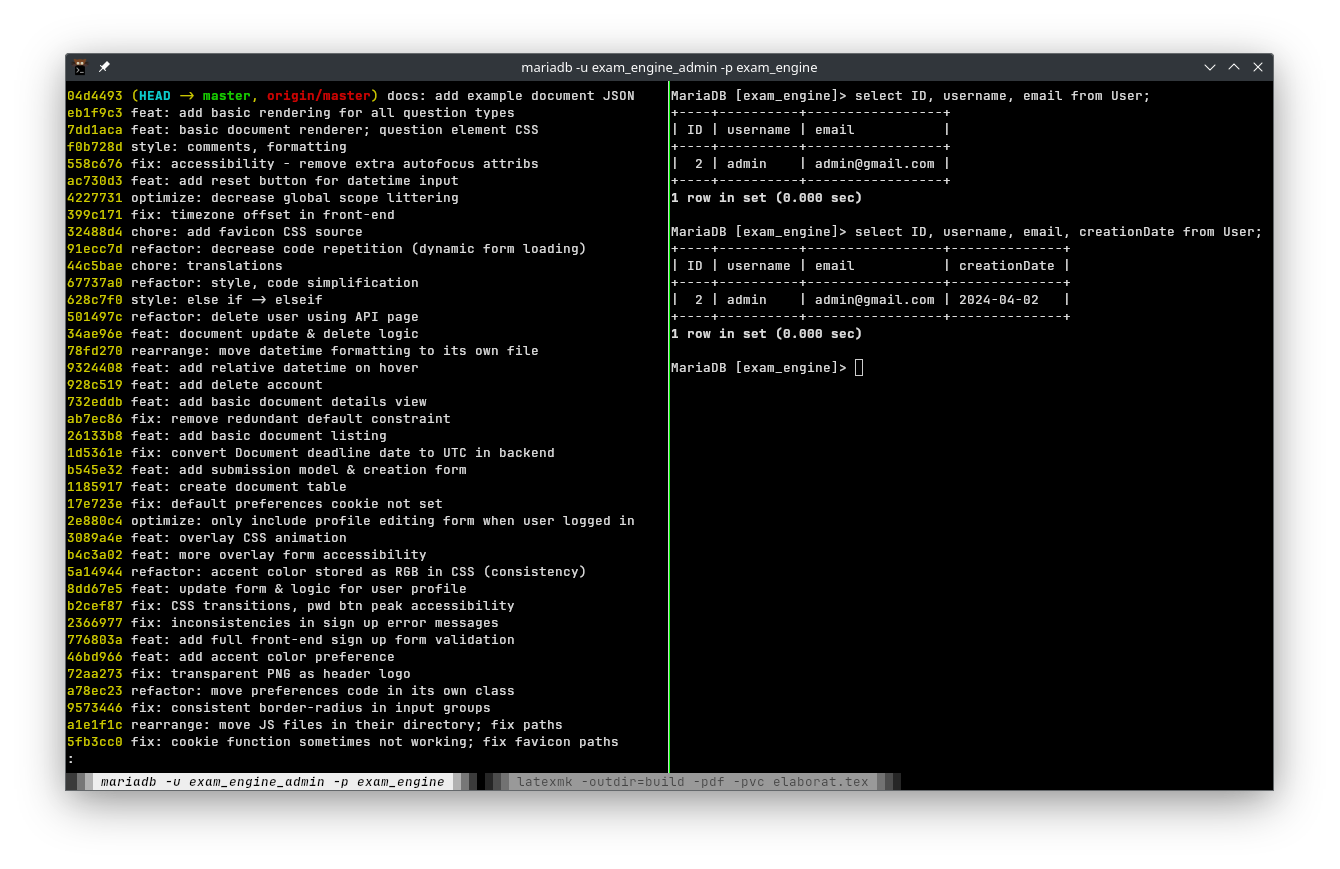
\includegraphics[width=\textwidth]{kitty}
      \caption{kitty terminal s više otvorenih kartica i panela.}
    \end{figure}

  \subsection{\textit{Web stack}}

    Aplikacija je razvijana na klasičnom \textit{LAMP} web stogu programske
    podrške (engl. \textit{web stack}) - Linux, Apache, MariaDB i PHP. Apache je
    popularan HTTP web server. MariaDB je popularan DBMS (engl. \textit{Database
    Management System}).

  \subsection{\textit{Web} preglednici}

    \begin{wrapfigure}{r}{0.5\textwidth}
      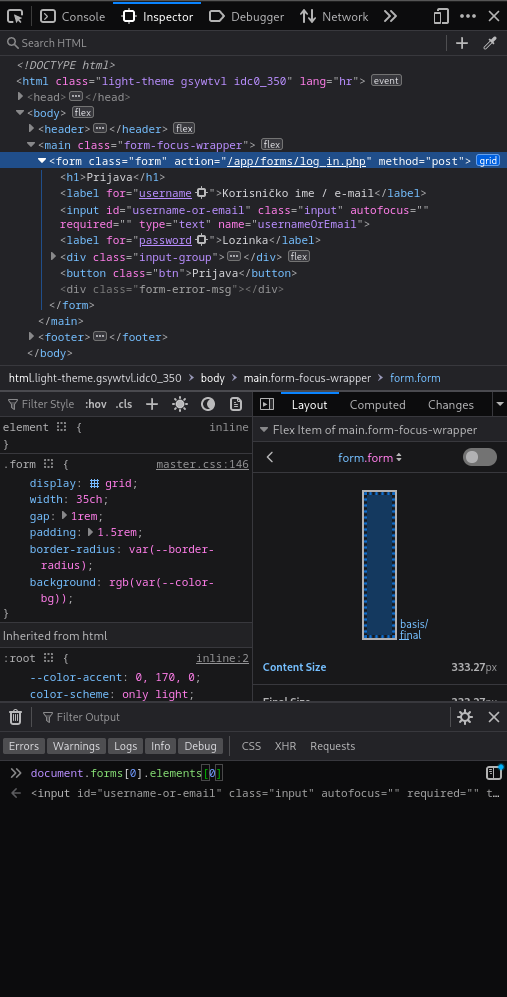
\includegraphics[width=\linewidth]{devtools}
      \caption{Alati za web programere, preglednik Mozilla Firefox.}
    \end{wrapfigure}

    Aplikacija je testirana na dvoje najpopularnijih web preglednika: Google
    Chrome i Mozilla Firefox. Potrebno je testirati na više preglednika radi
    konzistencije izgleda sučelja jer svaki preglednik ima malo drugačiju
    implementaciju HTML, CSS i JS standarda.

    Važno je spomenuti i integrirane alate za web programere koje nude oba web
    preglednika: inspektor (engl. \textit{inspector}), konzola (engl.
    \textit{console}), spremište (engl. \textit{storage}) itd.

  \subsection{Ostalo}

    \begin{itemize}
      \item JSON linter/validator/minifier: \\ \url{https://jsonlint.com/}
      \item regular expressions 101: \\ \url{https://regex101.com/}
      \item phpMyAdmin: \\ \url{https://www.phpmyadmin.net/}
      \item Fontovi: \\ \url{https://fonts.google.com/}
      \item Ikonice: \\ \url{https://icons.getbootstrap.com/}
    \end{itemize}

\section{Programski i ostali jezici}

  \subsection{\textit{Front-end}}

  Pod \textit{front-end} dio aplikacije spadaju sve stranice web aplikacije koje
  su vidljivi krajnjem korisniku/ci. Preko njih korisnik/ca upravlja i
  prosljeđuje podatke aplikaciji.

    \subsubsection*{\textit{HTML}}

      HTML (engl. \textit{HyperText Markup Language}) je označni jezik za
      definiranje osnovne strukture i sadržaja web dokumenata. Koristim aktualnu
      inačicu i standard \textit{HTML5}.

    \subsubsection*{\textit{CSS}}

      \textit{CSS} (engl. \textit{Cascading Style Sheets}) je jezik za
      oblikovanje i stiliziranje HTML dokumenata. Omogućava definiranje položaja
      elemenata, boje, fonta, efekata i sl. Koristim aktualnu inačicu i standard
      \textit{CSS3}.

    \subsubsection*{\textit{JavaScript}}

      \textit{JavaScript} (skraćeno \textit{JS}) je programski jezik za
      interakciju s korisnikom, razmjenu podataka i kreiranje dinamične,
      funkcionalne web stranice. Jezik je visoke razine, dinamički pisan, OO
      (objektno orijentiran) i interpretiran. Valja spomenuti i DOM (engl.
      \textit{Document Object Model}) pomoću kojeg je moguće dinamički
      manipulirati HTML-om i CSS-om dokumenta.

    \begin{figure}[h]
      \centering
      
\includegraphics[height=4cm]{front_end}
      \vspace{0.5cm}
      \caption{Front-end jezici.}
    \end{figure}

  \subsection{\textit{Back-end}}

    \subsubsection*{\textit{SQL (MariaDB)}}

      SQL (engl. \textit{Structured Query Language}) je deklarativni jezik koji
      služi za postavljanje upita (engl. \textit{query}) DBMS-u (bazi podataka).
      Upitima je moguće kreirati (engl. \textit{create}), čitati (engl.
      \textit{read}), ažurirati (engl. \textit{update}) i brisati (engl.
      \textit{delete}) podatke - tzv. CRUD operacije.

    \subsubsection*{\textit{PHP}}

      PHP je skriptni programski jezik koji se izvršava isključivo na
      poslužitelju. Jezik je visoke razine, dinamički pisan, OO (objektno
      orijentiran) i interpretiran. Služi za komuniciranje aplikacije s bazom
      podataka. Nakon izvršavanja na serveru, sav HTML izlaz PHP skripte šalje
      se klijentskom računalu i korisnik vidi gotovu stranicu.

    \begin{figure}[h]
      \centering
      
\includegraphics[width=\textwidth]{back_end}
      \caption{Back-end programski jezici i programska podrška.}
    \end{figure}

  \subsection{Ostalo}

    \subsubsection*{\textit{JSON}}

      JSON (JavaScript Object Notation) je tekstualni format za spremanje
      podataka. JSON zapisi razumljivi su i čovjeku i računalu (programu).

    \subsubsection*{\textit{LaTeX}}

      PDF dokument elaborata napravljen je pomoću označnog jezika \textit{LaTeX}
      i prevoditelja (engl. \textit{compiler}) \textit{latexmk}. Iz izvornog
      \textit{LaTeX} koda prevoditelj generira profesionalno formatirani i
      stilizirani PDF dokument.

\section{Arhitektura baze podataka}

  \subsection{Dizajn baze podataka}

    Baza podataka sastoji se od 2 tablice: \textit{User} -- korisnici i
    \textit{Document} -- dokumenti. Veza je 1:M (1 naprema više).

    Svaki zapis entiteta jedinstven je po svojem primarnom ključu (engl.
    \textit{primary key}, oznaka \textit{PK}). PK je broj koji se inkrementira
    za svaki novi zapis tog entiteta.

    Tablice se vezuju pomoću tzv. stranih ključeva (engl. \textit{foreign key},
    oznaka \textit{FK}). \textit{FK} pokazuje na odgovarajući \textit{PK} u
    nekoj drugoj tablici, i tipovi podataka im moraju biti identični.

    Većina atributa imaju i \textit{not null constraint}, što znači da
    vrijednosti tog atributa svakog zapisa u tablici treba biti poznat
    (definiran).

    Baza podataka je projektirana u skladu s prve 3 normalne forme (1NF, 2NF,
    3NF).

    \begin{figure}[h]
      \centering
      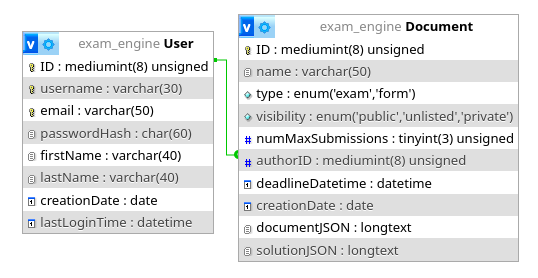
\includegraphics[scale=0.85]{model}
      \caption{Dijagram baze podataka prikazan u \textit{phpMyAdminu}.}
    \end{figure}

    \subsubsection{Tipovi podataka}

      Važno je kvalitetno odabrati tipove podatka atributa u tablicama tako da
      se uštedi na memoriji, ali ujedno osigura i buduća prilagodba i
      proširivost funkcionalnosti baze.

      Primjer toga je način korištenja char i varchar tipova podataka. Brojevi u
      zagradi (npr. \textit{varchar(40)}) označavaju najveći broj znakova u tom
      atributu. Također su korišteni i unsigned mediumint primarni ključevi da
      se dodatno uštedi na pohrani.

    \subsubsection{Entitet \textit{User}}

      Ova tablica služi za pohranu podataka o svakom registriranom korisniku.
      Čuvaju se: korisničko ime, e-mail, ime, prezime, datum registracije i
      datum i vrijeme zadnje prijave. Također postoji i atribut
      \textit{passwordHash}, koji sprema lozinku korisničkog računa, čime se
      ostvaruje autentikacija i autorizacija korisničkih podataka.

      Valja napomenuti da se prije pohrane u bazu sve lozinke procesiraju kroz
      jednosmjerni algoritam za tzv. \textit{hashiranje}, tj. kriptira se, što
      služi kao osnovna mjera zaštite korisničkih lozinka.

    \subsubsection{Entitet \textit{Document}}

      Ova tablica služi za pohranu podataka o dokumentima, tj. ispitima i
      obrascima. Čuvaju se: naziv dokumenta, tip, vidljivost, broj dozvoljenih
      pokušaja (predaja), autor dokumenta (FK), datum i vrijeme roka predaje i
      datum izrade.

      Atribut \textit{documentJSON} je tipa \textit{JSON} i služi za pohranu
      pitanja i sadržaja od kojih se sastoji svaki dokument.

      Atribut \textit{solutionJSON} pohranjuje samo rješenja dokumenta (ako je
      taj dokument tipa ispit). Kako bi aplikacija bila povjerljiva, iz
      sigurnosnih razloga, rješenja dokumenta (odgovori) su odvojena od samih
      pitanja.

    \subsection{\textit{SQL} skripta baze podataka}

      \subsubsection{Izrada MariaDB korisnika i baze podataka}

        \lstinputlisting[language=SQL, caption={
          SQL -- Izrada MariaDB korisnika i baze podataka.}]{01_setup.sql}

      \pagebreak[4]
      \subsubsection{Izrada i povezivanje tablica}

        \lstinputlisting[language=SQL, caption={
          SQL -- Izrada i povezivanje tablica.}]{02_schema.sql}


\section{Izvedba aplikacije}

  \subsection{PHP konfiguracija}

    Ova PHP skripta se obavezno \textit{includea} na vrhu svake druge PHP
    skripte. Sadrži neke osnovne PHP postavke.

    \lstinputlisting[language=PHP, alsolanguage=HTML, caption={
      PHP -- Osnovna konfiguracija}]{config.php}

  \subsection{Recikliranje koda}

    Jedan od temeljnih principa programiranja je izbjeći lošu redundanciju u
    kodu (engl. \textit{DRY - Don't Repeat Yourself.}). Iz tog razloga sam kod
    aplikacije pisao vrlo organizirano i modularno, te pokušavao definirati
    metode i funkcije za kod koji se ponavlja.

    Npr. postoje klase u projektu \textit{UserModel} i \textit{DocumentModel}.
    \textit{UserModel} sadrži sve metode i atribute koje opisuju korisnika.
    Slično vrijedi i za \textit{DocumentModel} klasu.

    \subsubsection{\textit{Util} klasa}

      \textit{Util} klasa (engl. \textit{Utility}) sadrži statičke metode koje
      se često koriste na raznim mjestima u projektu, ali ne mogu se
      kategorizirati u klasu za sebe.

      \lstinputlisting[language=PHP, alsolanguage=HTML, caption={
          PHP -- Util klasa}]{Util.php}

    \subsubsection{\textit{DB} klasa}

      \textit{DB} klasa (engl. \textit{DataBase}) sadrži često korištene metode
      i svojstva vezane za upravljanje bazom podataka, koje su smještene u tzv.
      \textit{singleton} klasu.

      \lstinputlisting[language=PHP, caption={
          PHP -- DB klasa}]{DB.php}

      \subsubsection{Jezik aplikacije}

        Višejezičnost aplikacije je postignuta tako da su svi znakovni nizovi
        korišteni u aplikaciji organizirani u dvije slične PHP datoteke -
        lang\_en.php i lang\_hr.php. Obje datoteke sadrže asocijativno polje
        \textit{LANG} -- ključevi su isti, a vrijednosti prevedene.

        \lstinputlisting[language=PHP, caption={
          PHP -- Engleski znakovni nizovi}]{lang_en.php}

        \lstinputlisting[language=PHP, caption={
          PHP -- Hrvatski znakovni nizovi}]{lang_hr.php}

    \subsubsection{Osnovna struktura stranice}

    \begin{figure}[h]
      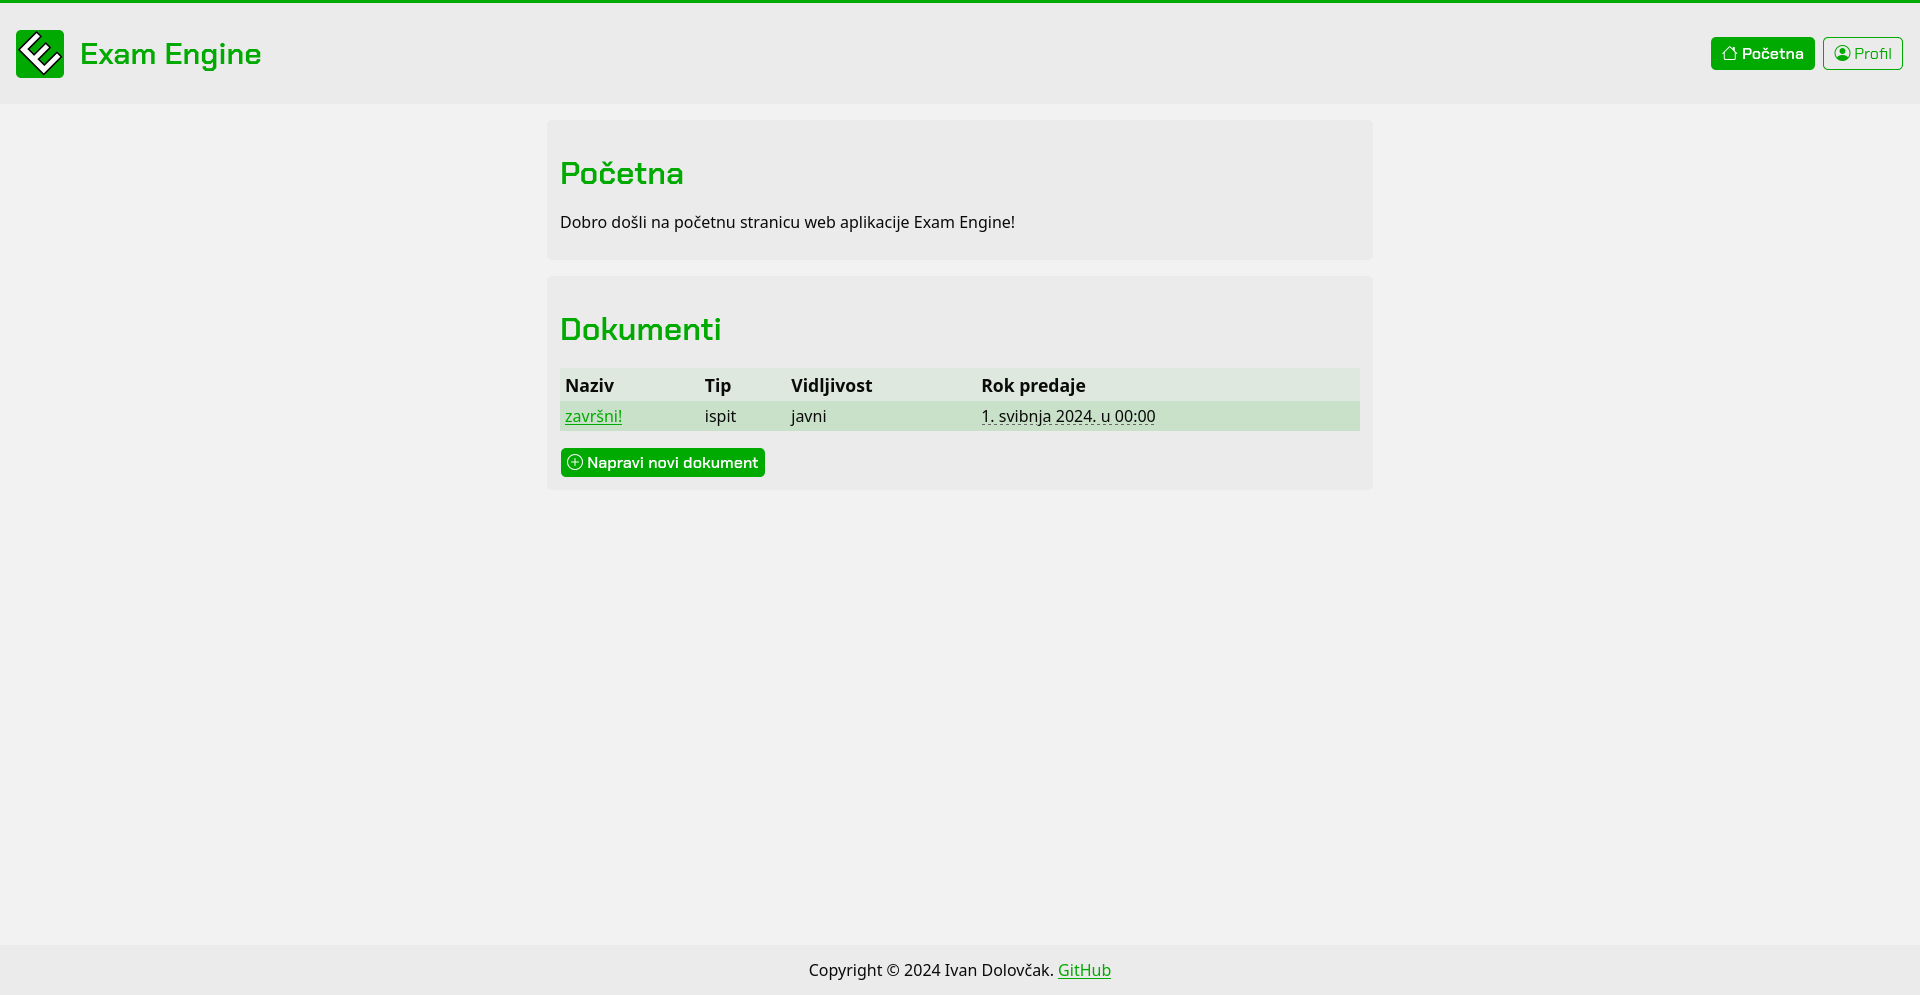
\includegraphics[width=\textwidth]{page_template}
      \caption{Početna stranica s popisom dokumenata.}
    \end{figure}

    Na svakoj stranici se ponavljaju zaglavlje i podnožje. Zaglavlje i podnožje
    stranice su stavljeni u zasebne datoteke (header.phtml i footer.phtml) te se
    na svakoj stranici \textit{includeaju}.

    Zaglavlje sadržava logotip aplikacije, naslov i navigator s poveznicama koje
    vode do glavnih stranica (engl. \textit{views}) aplikacije. Navigator
    mijenja svoj sadržaj ovisno o tome je li korisnik prijavljen. Ako nije,
    prikazuju se poveznice za registraciju i prijavu. Ako je, onda su te
    poveznice sakrivene.

    \begin{figure}[h]
      \centering
      
\includegraphics[scale=0.4]{header}
      \caption{Navigator kad korisnik nije prijavljen.}
    \end{figure}

    \subsection{Korisničke postavke (\textit{front-end})}

      \begin{figure}[h]
        \begin{center}
          \begin{subfigure}{0.65\textwidth}
            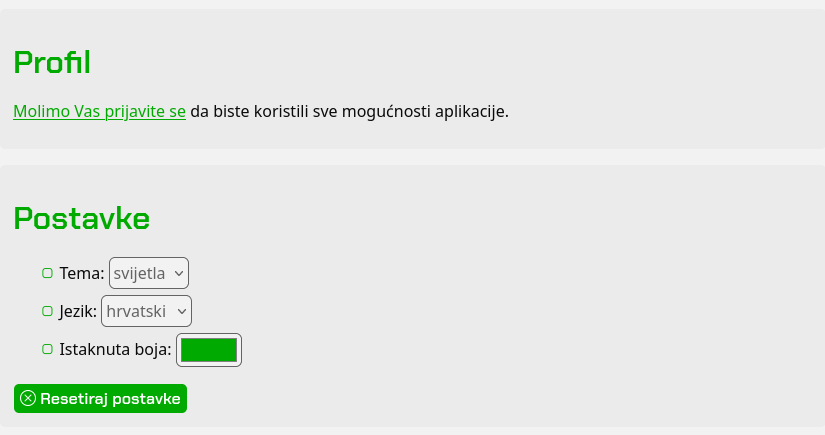
\includegraphics[width=\linewidth]{page_preferences_1}
          \end{subfigure}
          \\
          \begin{subfigure}{0.65\textwidth}
            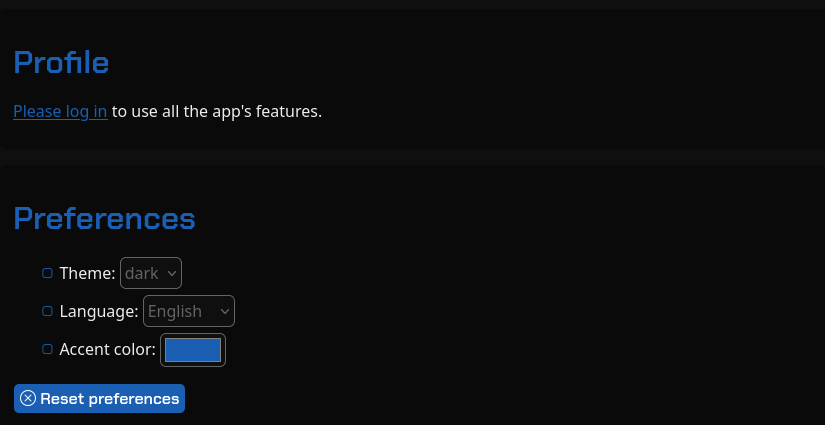
\includegraphics[width=\linewidth]{page_preferences_2}
          \end{subfigure}

          \caption{Prilagodljivost sučelja (profile.phtml)}
        \end{center}
      \end{figure}

      Izgled sučelja aplikacije je prilagodljiv korisniku.
      Korisničke postavke (engl. \textit{Preferences}) sastoje se od:

      \begin{itemize}
        \item teme (svijetla ili tamna),
        \item jezika (engleski ili hrvatsi)
        \item i boje isticanja (proizvoljna).
      \end{itemize}


    \subsection{Korisničke postavke (\textit{back-end})}

      Da bi mijenjao ove postavke prikaza, korisnik ne mora biti
      prijavljen u aplikaciju, jer se ove postavke spremaju u tzv. kolačić
      (engl. \textit{cookie}). Ako kolačić ne postoji (prva posjeta \textit{web}
      sjedištu), dodjeljuju se zadane (\textit{defaultne}) postavke (svijetla
      tema, zelena boja isticanja, engleski jezik).

      \subsubsection{\textit{Preferences} klasa}

        \lstinputlisting[language=PHP, caption={
          PHP -- Preferences klasa}]{Preferences.php}

  \subsection{Registracija korisnika (\textit{front-end})}

    \subsubsection{Prikaz obrasca za registraciju}

      \begin{figure}[h]
          \begin{subfigure}{0.5\textwidth}
            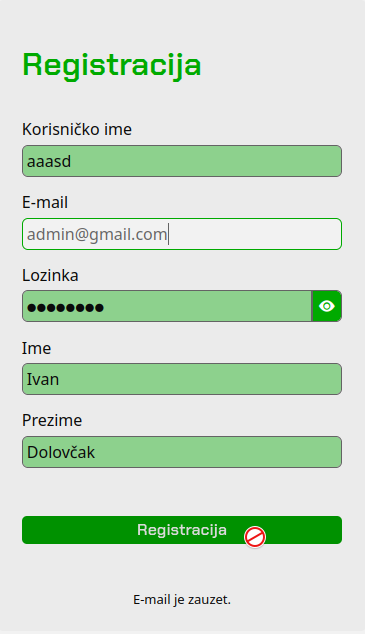
\includegraphics[width=0.9\linewidth]{form_register_1}
          \end{subfigure}
          \begin{subfigure}{0.5\textwidth}
            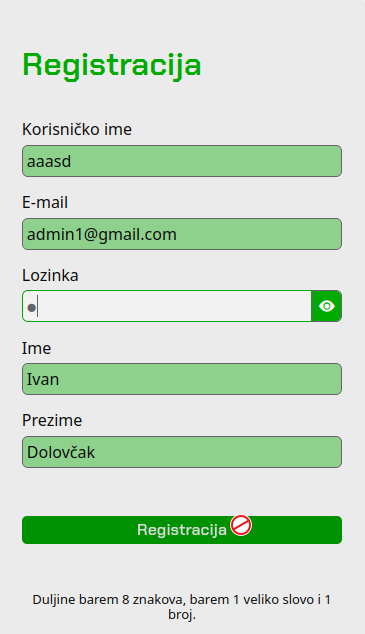
\includegraphics[width=0.9\linewidth]{form_register_2}
          \end{subfigure}

          \caption{Obrazac za registraciju -- validacija u realnom vremenu}
      \end{figure}

      Kako bi koristio sve mogućnosti aplikacije, korisnik mora biti
      registriran. To obavlja preko ovog obrasca, koji je intuitivan jer ima
      ugrađenu tzv. \textit{front-end} validaciju.

      Također, desno od polja za unos lozinke nalazi se gumb za prikazivanje
      lozinke. Lozinka se prikazuje samo kad korisnik drži gumb pritisnutim,
      inače je lozinka skrivena. To je postignuto trivijalnim JS kodom.

      Sva polja moraju biti popunjena i ispravna. Ukoliko neko polje nije ispravno,
      na dnu obrasca se u realnom vremenu (prije podnašanja obrasca) prikazuje
      povratna informacija korisniku te mu nije dozvoljeno podnašanje
      obrasca.

      Ukoliko je ispravno, polje se blago osjenča zelenom bojom. Ovo su uvjeti za
      ispravnost polja:

      \begin{itemize}
        \item Korisničko ime: Koristite velika i mala slova bez dijakritičkih
        znakova, brojeve i donje crte, duljine najmanje 4 znakova.
        \item Lozinka: Duljine barem 8 znakova, barem 1 veliko slovo i 1 broj.
        \item Ime i prezime: Duljine najmanje 3 znakova, bez brojeva.
        \item Korisničko ime i e-mail adresa ne smiju biti zauzeti
      \end{itemize}

      Valja napomenuti da su tijekom dizajniranja \textit{front-enda} uzete u
      obzir osnovne prakse pristupačnosti (engl. \textit{accessibility}):
      autofocus atributi, korištenje label elemenata koji su povezani sa svojim
      poljima za unos, te je za svako polje sačuvan tabindex atribut.

      \subsubsection{HTML/PHP struktura obrasca registracije}

        \lstinputlisting[language=PHP, alsolanguage=HTML, caption={
          HTML/PHP -- Obrazac za registraciju.}]{form_sign_up.phtml}

      \subsubsection{JS kod za validaciju}

        \lstinputlisting[language=JavaScript, caption={
          JS -- Live validacija forme.}]{form_validation.js}

  \subsection{Registracija korisnika (\textit{back-end})}

    \textit{Front-end} validaciju vrlo je lako zaobići, stoga je iz
    sigurnosnih razloga potrebno obaviti validaciju i u \textit{back-end}
    dijelu aplikacije.

    \subsubsection{Obrada obrasca za registraciju}

      \lstinputlisting[language=PHP, caption={
        PHP -- Obrada obrasca za registraciju.}]{sign_up.php}

    \subsubsection{Spremanje korisnika u bazu podataka}

      \lstinputlisting[language=PHP, alsolanguage=HTML, caption={
        PHP/SQL -- Spremanje korisnika u bazu podataka.}]{UserModelsignUp.php}

  \subsection{Prijava korisnika}

    \begin{figure}[h]
      \begin{subfigure}{0.5\textwidth}
        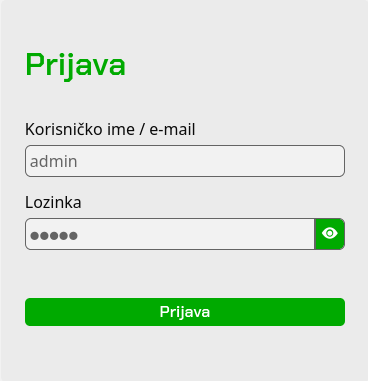
\includegraphics[width=0.9\linewidth]{form_login_1}
      \end{subfigure}
      \begin{subfigure}{0.5\textwidth}
        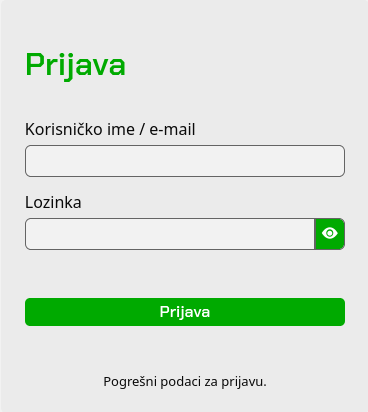
\includegraphics[width=0.9\linewidth]{form_login_2}
      \end{subfigure}

      \caption{Obrazac za prijavu}
    \end{figure}

    Korisnik se može prijaviti ili korisničkim imenom ili e-mail adresom.
    HTML kod i PHP kod za validaciju je nepotrebno pokazivati jer su vrlo slični
    kodu svakog drugog obrasca u projektu.

    Ako je lozinka pogrešna, prikazuje se greška korisniku na dnu obrasca.

    \lstinputlisting[language=PHP, alsolanguage=HTML, caption={
        PHP -- Prijava korisnika}]{UserModelLogIn.php}

  \subsection{Profil korisnika}

    \begin{figure}[h]
      
\includegraphics[width=\textwidth]{page_profile}
      \caption{Stranica s profilom korisnika.}
    \end{figure}

    Na ovoj stranici nalaze se detalji korisničkog računa. Također, ako je
    korisnik prijavljen, prikazuju se gumbi za odjavu, uređivanje detalja
    profila i brisanje samog profila.

    Klikom na gumb za odjavu uništava se sesija i preusmjerava se na obrazac za
    prijavu.

    \lstinputlisting[language=PHP, alsolanguage=HTML, caption={
        PHP -- Odjava korisnika.}]{log_out.php}

    Klikom na gumb za brisanje računa otvara se skočni modalni prozor (engl.
    \textit{overlay}) za potvrdu brisanja. Ako korisnik potvrdi, briše se račun
    i svi dokumenti korisnika.

    \lstinputlisting[language=PHP, alsolanguage=HTML, caption={
      PHP/SQL -- Brisanje korisnika.}]{UserModelDelete.php}

    \begin{figure}[h]
      \centering
      
\includegraphics[width=0.5\textwidth]{delete_profile}
      \caption{Skočni modalni prozor za potvrdu brisanja računa.}
    \end{figure}

    Klikom na gumb za uređivanje profila, otvara se isti obrazac kao za
    registraciju korisnika (osim polja za lozinku) -- HTML struktura i kod za
    validaciju se reciklira. Razlika je u tome što se ovaj obrazac prikazuje u
    \textit{overlayu}. Polja se popune s vrijednostima u bazi podataka.

    \begin{figure}[h]
      \centering
      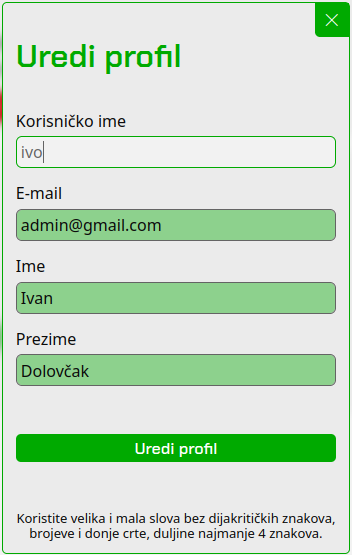
\includegraphics[width=0.5\textwidth]{form_edit_profile}
      \caption{Skočni modalni prozor za uređivanje profila.}
    \end{figure}

  \subsection{Početna stranica (\textit{front-end})}

    \subsubsection{Popis dokumenata}

      Na početnoj stranici su tabelarno prikazani svi dokumenti korisnika te
      njihovi detalji. Klikom na poveznicu u prvom stupcu tablice preusmjerava na
      stranicu detalja dokumenata, gdje su prikazani svi detalji dokumenta.
      Prelaskom miša (engl. \textit{hover}) preko datuma roka (ako je definiran)
      prikazuje se u malom prozoru (engl. \textit{tooltip}) \textit{relativan}
      datum.

      \begin{figure}[h]
        \centering
        \begin{subfigure}{\textwidth}
          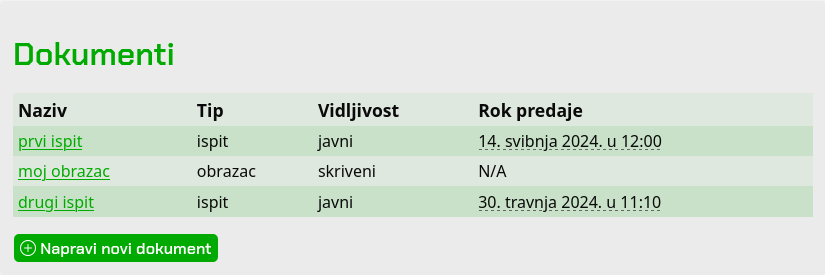
\includegraphics[width=0.9\linewidth]{documents_list}
        \end{subfigure}
        \\
        \begin{subfigure}{\textwidth}
          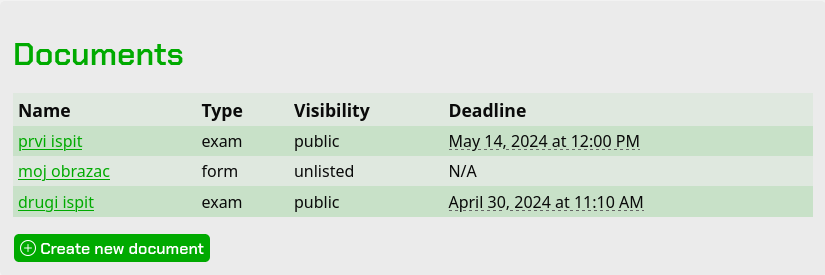
\includegraphics[width=0.9\linewidth]{documents_list_en}
        \end{subfigure}

        \caption{Popis dokumenata; višejezičnost.}
      \end{figure}


\section{Zaključak}

  Elaborat završnog rada dokumentira arhitekturu i programsku izvedbu web
  aplikacije za kreiranje i rješavanje ispita i obrazaca. Korisnik/ca može nakon
  prijave kreirati svoje dokumente i rješavati tuđe. Korisnik/ca vidi popise
  vlastitih i tuđih dokumenata i rješenja tih dokumenata. Moguće je uređivanje
  detalja i brisanje vlastitog profile i vlastitih dokumenata. Korisnik/ca može
  prilagoditi sučelje aplikacije svojim potrebama. Sučelje aplikacije je
  intuitivno i pristupačno.

  Prilikom izvedbe web aplikacije korišteni su moderni JavaScript API-ji: Fetch,
  DOM i Intl. PHP nudi MySQLi API za upravljanje bazom podataka. U PHP-u sam
  također koristio kolačiće i varijable sesije. I JavaScript i PHP kod pretežito
  koriste OOP model programiranja.

  Zahvaljujući modularnosti koda i kvalitetnim komentarima, aplikaciju je
  jednostavno proširiti. U budućnosti bih preveo aplikaciju na više jezika,
  dodao prijavu pomoću Google API-ja, dodao još različitih tipova pitanja te
  dotjerao \textit{front-end} da bude još profesionalnijeg izgleda.

  Nastojao sam pisati dobro organiziran, siguran, moderan, kvalitetno
  dokumentiran, efikasan i modularan izvorni kod -- koliko je god bilo moguće.
  Ovo mi je najopširniji programerski projekt do sad. Naučio sam jako puno
  korisnih stvari vezanih uz struku i predmet te uveliko proširio znanje i
  vještine stečene u školi.

\listoffigures

\lstlistoflistings
\addcontentsline{toc}{section}{\lstlistlistingname}

\section*{Literatura}
\addcontentsline{toc}{section}{Literatura}

  \begin{itemize}
    \item \textit{Stack Overflow} - web sjedište sa pitanjima i odgovorima za
      profesionalne programere: \url{https://stackoverflow.com/}
    \item \textit{PHP} priručnik: \url{https://www.php.net/manual/en/}
    \item \textit{MDN Web Docs} - priručnik za \textit{HTML}, \textit{CSS} i
      \textit{JavaScript}: \\\url{https://developer.mozilla.org/en-US/}
    \item \textit{MariaDB SQL} dokumentacija:
      \url{https://mariadb.com/kb/en/documentation/}
    \item \textit{Apache} dokumentacija: \url{https://httpd.apache.org/docs/2.4/}
  \end{itemize}

\cleardoublepage
\section*{Konzultacijski list učenika \hfill Razredni odjel: 4.AT}


\begin{table}[h]
      \subsubsection*{Konzultacije s mentorom:}

      \def\arraystretch{1.6}
      \footnotesize

      \centering
      \begin{tabularx}{\textwidth}{|r|X|l|l|}
      \cline{1-4}
      \textbf{RB} & \textbf{Sadržaj (bilješke o napredovanju)} & \textbf{Potpis mentora} & \textbf{Datum} \\ \cline{1-4}
      1. & Mentor prihvatio predloženu temu rada  &                & 27.10.2023. \\ \cline{1-4}
      2. & Poslana poveznica za GitHub repozitorij  &                & 15.01.2024. \\ \cline{1-4}
      3. & Konfiguracija hostinga &                & 23.02.2024. \\ \cline{1-4}
      4. & Savjeti za pisanje elaborata  &   &  25.04.2024. \\ \cline{1-4}
      5. & Slanje prve inačice elaborata mentoru na uvid  &                &   01.05.2024.    \\ \cline{1-4}
      \end{tabularx}
    \end{table}

    \begin{center}
      \vspace{-0.5cm}
      \begin{tabular}{@{}l@{}}
        Datum predaje rada: \rule{3cm}{0.5pt} \\
        Potpis mentora: \rule{4cm}{0.5pt} \scriptsize{(mentor je prihvatio izradbu)}\normalsize \\
        Ocjena pisanog rada: \rule{4cm}{0.5pt} \\
        Datum obrane rada: \rule{3cm}{0.5pt} \\
        Ocjena obrane rada: \rule{4cm}{0.5pt} \\
        \textbf{Konačna ocjena: \rule{4cm}{0.5pt}}
        \vspace{-0.5cm}
      \end{tabular}
      % \mbox{Datum predaje rada: \rule{4cm}{0.5pt} \hfill Potpis mentora: \rule{4cm}{0.5pt} }

      % \mbox{Ocjena pisanog rada: \rule{6cm}{0.5pt}}


      % \mbox{Konačna ocjena: \rule{6cm}{0.5pt}}
    \end{center}

  \subsubsection*{Povjerenstvo:}

    % Set the width of the text into \mytextwidth
    \settowidth{\mytextwidth}{mentor: }

    % Define the length of the line
    \setlength{\myline}{\mytextwidth}

    \begin{enumerate}
      \item mentor: \rule{6.5cm}{0.5pt}
      \item \rule{\myline+6.5cm}{0.5pt}
      \item \rule{\myline+6.5cm}{0.5pt}
      \item \rule{\myline+6.5cm}{0.5pt}
      \item \rule{\myline+6.5cm}{0.5pt}
    \end{enumerate}

  \subsubsection*{Komentar:}

    \framebox[\textwidth][c]{\rule{0pt}{4.1cm}}


\end{document}
